% Options for packages loaded elsewhere
\PassOptionsToPackage{unicode}{hyperref}
\PassOptionsToPackage{hyphens}{url}
%
\documentclass[
]{article}
\usepackage{amsmath,amssymb}
\usepackage{lmodern}
\usepackage{ifxetex,ifluatex}
\ifnum 0\ifxetex 1\fi\ifluatex 1\fi=0 % if pdftex
  \usepackage[T1]{fontenc}
  \usepackage[utf8]{inputenc}
  \usepackage{textcomp} % provide euro and other symbols
\else % if luatex or xetex
  \usepackage{unicode-math}
  \defaultfontfeatures{Scale=MatchLowercase}
  \defaultfontfeatures[\rmfamily]{Ligatures=TeX,Scale=1}
\fi
% Use upquote if available, for straight quotes in verbatim environments
\IfFileExists{upquote.sty}{\usepackage{upquote}}{}
\IfFileExists{microtype.sty}{% use microtype if available
  \usepackage[]{microtype}
  \UseMicrotypeSet[protrusion]{basicmath} % disable protrusion for tt fonts
}{}
\makeatletter
\@ifundefined{KOMAClassName}{% if non-KOMA class
  \IfFileExists{parskip.sty}{%
    \usepackage{parskip}
  }{% else
    \setlength{\parindent}{0pt}
    \setlength{\parskip}{6pt plus 2pt minus 1pt}}
}{% if KOMA class
  \KOMAoptions{parskip=half}}
\makeatother
\usepackage{xcolor}
\IfFileExists{xurl.sty}{\usepackage{xurl}}{} % add URL line breaks if available
\IfFileExists{bookmark.sty}{\usepackage{bookmark}}{\usepackage{hyperref}}
\hypersetup{
  pdftitle={Практическая работа №1},
  pdfauthor={Фёдорова В. Р.},
  hidelinks,
  pdfcreator={LaTeX via pandoc}}
\urlstyle{same} % disable monospaced font for URLs
\usepackage[margin=1in]{geometry}
\usepackage{longtable,booktabs,array}
\usepackage{calc} % for calculating minipage widths
% Correct order of tables after \paragraph or \subparagraph
\usepackage{etoolbox}
\makeatletter
\patchcmd\longtable{\par}{\if@noskipsec\mbox{}\fi\par}{}{}
\makeatother
% Allow footnotes in longtable head/foot
\IfFileExists{footnotehyper.sty}{\usepackage{footnotehyper}}{\usepackage{footnote}}
\makesavenoteenv{longtable}
\usepackage{graphicx}
\makeatletter
\def\maxwidth{\ifdim\Gin@nat@width>\linewidth\linewidth\else\Gin@nat@width\fi}
\def\maxheight{\ifdim\Gin@nat@height>\textheight\textheight\else\Gin@nat@height\fi}
\makeatother
% Scale images if necessary, so that they will not overflow the page
% margins by default, and it is still possible to overwrite the defaults
% using explicit options in \includegraphics[width, height, ...]{}
\setkeys{Gin}{width=\maxwidth,height=\maxheight,keepaspectratio}
% Set default figure placement to htbp
\makeatletter
\def\fps@figure{htbp}
\makeatother
\setlength{\emergencystretch}{3em} % prevent overfull lines
\providecommand{\tightlist}{%
  \setlength{\itemsep}{0pt}\setlength{\parskip}{0pt}}
\setcounter{secnumdepth}{-\maxdimen} % remove section numbering
\ifluatex
  \usepackage{selnolig}  % disable illegal ligatures
\fi

\title{Практическая работа №1}
\author{Фёдорова В. Р.}
\date{10/9/2021}

\begin{document}
\maketitle

\hypertarget{ux432ux438ux434ux44b-ux430ux43dux430ux43bux438ux437ux430-ux434ux430ux43dux43dux44bux445}{%
\section{Виды анализа
данных}\label{ux432ux438ux434ux44b-ux430ux43dux430ux43bux438ux437ux430-ux434ux430ux43dux43dux44bux445}}

\hypertarget{ux43cux435ux445ux430ux43dux438ux441ux442ux438ux447ux435ux441ux43aux438ux439-ux430ux43dux430ux43bux438ux437}{%
\subsubsection{1. Механистический
анализ}\label{ux43cux435ux445ux430ux43dux438ux441ux442ux438ux447ux435ux441ux43aux438ux439-ux430ux43dux430ux43bux438ux437}}

\textbf{Цель} данного вида анализа состоит в определении конкретных
измнений в переменных, которые влекут за собой точные изменения в других
переменных.

Механистический анализ применяется в следующих случаях:

\begin{itemize}
\item
  Простые случаи;
\item
  Ситуации, которые хорошо моделируются детерминированными уравнениями;
\item
  В физических и инженерных науках.
\end{itemize}

Рассмотрим пример исследования, проведенного с помощью механистического
анализа:

\textbf{УДК 532.526}

\textbf{DOI 10.25205/2541-9447-2021-16-1-44-52}

\emph{В.Л.Кочарин ,Н.В.Семёнов ,А.Д.Косинов ,А.А.Яцких}

Институт теоретической и прикладной механики им С. А. Христиановича СО
РАН Новосибирск, Россия

\hypertarget{ux44dux43aux441ux43fux435ux440ux438ux43cux435ux43dux442ux430ux43bux44cux43dux43eux435-ux438ux441ux441ux43bux435ux434ux43eux432ux430ux43dux438ux435-ux432ux43bux438ux44fux43dux438ux44f-ux435ux434ux438ux43dux438ux447ux43dux43eux433ux43e-ux447ux438ux441ux43bux430-ux440ux435ux438ux43dux43eux43bux44cux434ux441ux430-ux43dux430-ux43fux43eux43bux43eux436ux435ux43dux438ux435-ux43bux430ux43cux438ux43dux430ux440ux43dux43e-ux442ux443ux440ux431ux443ux43bux435ux43dux442ux43dux43eux433ux43e-ux43fux435ux440ux435ux445ux43eux434ux430-ux43dux430-ux43aux440ux44bux43bux435-ux441-ux434ux43eux437ux432ux443ux43aux43eux432ux43eux438-ux43fux435ux440ux435ux434ux43dux435ux438-ux43aux440ux43eux43cux43aux43eux438-ux43fux440ux438-ux447ux438ux441ux43bux435-ux43cux430ux445ux430-2}{%
\subparagraph{\texorpdfstring{\emph{Экспериментальное исследование
влияния единичного числа Рейнольдса на положение ламинарно-турбулентного
перехода на крыле с дозвуковой передней кромкой при числе Маха
2}}{Экспериментальное исследование влияния единичного числа Рейнольдса на положение ламинарно-турбулентного перехода на крыле с дозвуковой передней кромкой при числе Маха 2}}\label{ux44dux43aux441ux43fux435ux440ux438ux43cux435ux43dux442ux430ux43bux44cux43dux43eux435-ux438ux441ux441ux43bux435ux434ux43eux432ux430ux43dux438ux435-ux432ux43bux438ux44fux43dux438ux44f-ux435ux434ux438ux43dux438ux447ux43dux43eux433ux43e-ux447ux438ux441ux43bux430-ux440ux435ux438ux43dux43eux43bux44cux434ux441ux430-ux43dux430-ux43fux43eux43bux43eux436ux435ux43dux438ux435-ux43bux430ux43cux438ux43dux430ux440ux43dux43e-ux442ux443ux440ux431ux443ux43bux435ux43dux442ux43dux43eux433ux43e-ux43fux435ux440ux435ux445ux43eux434ux430-ux43dux430-ux43aux440ux44bux43bux435-ux441-ux434ux43eux437ux432ux443ux43aux43eux432ux43eux438-ux43fux435ux440ux435ux434ux43dux435ux438-ux43aux440ux43eux43cux43aux43eux438-ux43fux440ux438-ux447ux438ux441ux43bux435-ux43cux430ux445ux430-2}}

\href{https://journals.nsu.ru/upload/iblock/996/0720_SJP_21T16V1_p44_p52.pdf}{Ссылка
на статью}

В данной статье проведены экспериментальные исследования влияния
единичного числа Рейнольдса на ламинарно-турбулентный переход в
сверхзвуковом пограничном слое скользящего крыла с дозвуковой передней
кромкой при числе Маха 2. Полученные термоанемометрические данные
показали, что ламинарно-турбулентный переход в сверхзвуковом пограничном
слое скользящего крыла с дозвуковой передней кромкой наступает раньше,
чем на модели со сверхзвуковой передней кромкой при одних и тех же
параметрах набегающего потока. Показано, что изменение единичного числа
Рейнольдса набегающего потока слабо влияет на ламинарно-турбулентный
переход в пограничном слое скользящего крыла с дозвуковой передней
кромкой.

Данное исследование использует механистический анализ, так как цель
исследования - понять как именно необходимо изменить единичное число
Рейнольдса для того, чтобы достичь точного изменения в положении
ламинарно-турбулентного перехода на крыле с дозвуковой передней кромкой
при числе Махa 2.

\begin{quote}
Выполнено экспериментальное исследование влияния единичного числа
Рейнольдса на положение ламинарно-турбулентного перехода в трехмерном
сверхзвуковом пограничном слое на модели скользящего крыла с углом
скольжения 72 градуса, что соответствует случаю дозвуковой передней
кромки при \(М = 2\).
\end{quote}

\begin{figure}
\centering
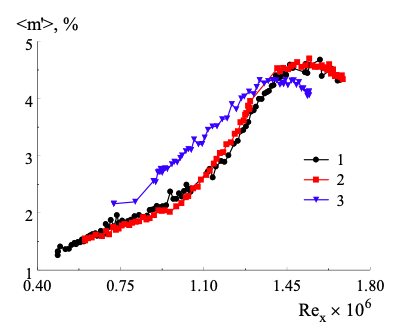
\includegraphics{image1.png}
\caption{Рис. 1. Зависимость среднеквадратичных пульсаций массового
расхода от числа Рейнольдса при М = 2.}
\end{figure}

\begin{quote}
Незначительное влияние числа \(Re_1\) было зафиксировано при измерениях
среднеквадратичных пульсаций массового расхода вниз по потоку при
\(\rho U \approx const\) для значений \(Re_1 = 14 × 10^6\) и
\(18 × 10^6 м^{–1}\)(рис. 2)
\end{quote}

\begin{figure}
\centering
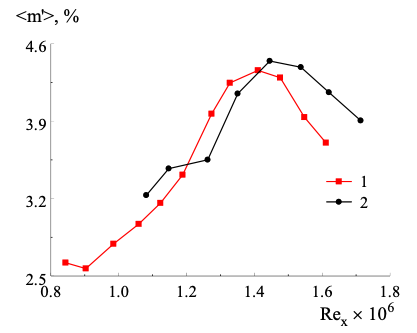
\includegraphics{image2.png}
\caption{Рис. 2. Зависимость среднеквадратичных пульсаций массового
расхода от числа Рейнольдса.}
\end{figure}

\hypertarget{ux440ux430ux437ux432ux435ux434ux43eux447ux43dux44bux439-ux430ux43dux430ux43bux438ux437}{%
\subsubsection{2. Разведочный
анализ}\label{ux440ux430ux437ux432ux435ux434ux43eux447ux43dux44bux439-ux430ux43dux430ux43bux438ux437}}

\textbf{Цель} разведочного анализа - изучить данные и найти взаимосвязи,
о которых ранее было неизвестно.

Разведочный анализ обладает следущими свойствами:

\begin{enumerate}
\def\labelenumi{\arabic{enumi}.}
\tightlist
\item
  Изучает, как могут быть связаны различные переменные;
\item
  Полезен для выявления новых связей;
\item
  Помогает сформулировать гипотезы и управлять планированием будущих
  исследований.
\end{enumerate}

Рассмотрим пример исследования, в котором используется разведочный
анализ:

\textbf{УДК 338}

\textbf{JEL 025}

\textbf{DOI 10.25205/2542-0429-2020-20-1-5-19}

\emph{В.А.Бажанов ,И.И.Орешко ,Л.С.Веселая}

Институт экономики и организации промышленного производства СО РАН
Новосибирск, Россия

Новосибирский национальный исследовательский государственный университет

\hypertarget{ux43eux446ux435ux43dux43aux430-ux44dux43aux441ux43fux43eux440ux442ux43dux44bux445-ux432ux43eux437ux43cux43eux436ux43dux43eux441ux442ux435ux438-ux43cux430ux448ux438ux43dux43eux441ux442ux440ux43eux435ux43dux438ux44f-ux432-ux440ux43eux441ux441ux438ux438}{%
\subparagraph{\texorpdfstring{\emph{Оценка экспортных возможностей
машиностроения в
России}}{Оценка экспортных возможностей машиностроения в России}}\label{ux43eux446ux435ux43dux43aux430-ux44dux43aux441ux43fux43eux440ux442ux43dux44bux445-ux432ux43eux437ux43cux43eux436ux43dux43eux441ux442ux435ux438-ux43cux430ux448ux438ux43dux43eux441ux442ux440ux43eux435ux43dux438ux44f-ux432-ux440ux43eux441ux441ux438ux438}}

\href{https://journals.nsu.ru/upload/iblock/697/01\%20(1).pdf}{Ссылка на
статью}

В данной статье осуществлена попытка оценки возможных параметров
состояния машиностроения в России в случае существенного увеличения
экспорта его продукции, предусмотренного национальным проектом
«Международная кооперация и экспорт». Оценка параметров основывается на
посылке, что увеличение экспорта машиностроительной продукции повлечет
за собой увеличение объемов ее производств в стране, что, в свою
очередь, вызовет необходимость возможного перевооружения и реконструкции
действующих производств и создание новых.

Так как в данном исследовании осуществляется попытка оценки возможных
параметров состояния машиностроения в России в случае существенного
увеличения экспорта, то есть производится поиск новых взаимосвязей в
машиностроении, о которых ранее не было известно, а также данное
исследование помогает сформулировать гипотезы в производстве при
возможном увеличении экспорта и спланировать дальнейшие действия в
отрасли машиностроения, то можно сказать, что в данной работе
использовался разведочный анализ.

Результаты расчетов эффектов от увеличения экспорта продукции
машиностроения в миллиардах рублей представлены в таблице:

\begin{longtable}[]{@{}
  >{\centering\arraybackslash}p{(\columnwidth - 10\tabcolsep) * \real{0.17}}
  >{\centering\arraybackslash}p{(\columnwidth - 10\tabcolsep) * \real{0.17}}
  >{\centering\arraybackslash}p{(\columnwidth - 10\tabcolsep) * \real{0.17}}
  >{\centering\arraybackslash}p{(\columnwidth - 10\tabcolsep) * \real{0.17}}
  >{\centering\arraybackslash}p{(\columnwidth - 10\tabcolsep) * \real{0.17}}
  >{\centering\arraybackslash}p{(\columnwidth - 10\tabcolsep) * \real{0.17}}@{}}
\toprule
Показатель & Химический комплекс & Металлургия и готовые изделия &
Производство машин & Торговля & Транспорт и связь \\
\midrule
\endhead
Валовая добавленная стоимость & 2665,0 & 2057,8 & 2741,7 & 12518,9 &
6033,2 \\
Выпуск отраслей в основных ценах & 10777,1 & 6338,2 & 8414,2 & 21635,9 &
12903,8 \\
Основные фонды в базовом году & 4308,7 & 2615,6 & 2749,9 & 4891,5 &
42493,6 \\
\bottomrule
\end{longtable}

\end{document}
